\textbf{Question: Assume a full-scale sinusoidal input with $f_0 = 37.1094 MHz$, and let the FFT size be M = 1024.
    Generate $15 \cdot M$ samples of $x(t)$ (at fs = 100 MHz) and quantize them to N = 12 bits. Break
    the vector xq of quantized samples into 15 size-M blocks using, e.g., the command reshape:}

\vspace{0.5cm}

\begin{lstlisting}[language=Matlab]
    xqblocks = reshape(xq, M, 15);
\end{lstlisting}

\textbf{so that each column of the $M \times 15$ matrix xqblocks will contain the corresponding block of size
    M . Now, since the fft command computes the FFT columnwise, in order to apply an M -point
    FFT to each block, we simply make
}
\begin{lstlisting}[language=Matlab]
    X = fft(xqblocks, M);
\end{lstlisting}

\textbf{Average the squared magnitude of the DFT coefficients over the 15 blocks and plot the results
    between 0 and fs/2, in dBFS.
    Observe the location and peak value of the principal frequency component, as well as the value
    of the noise floor. Do your observations agree (quantitatively) with what you would expect?
}
\vspace{0.5cm}

\subsection{Theoretical values}
First, we need to calculate the expected theoretical values for the signal peak and for the noise floor value.
\subsubsection{Signal Peak}
We have $f_0 = 37.1094 MHz$ and $f_s = 100 MHz$. As $f_0 < f_s/2$ we don't have aliasing.
Terefore, we expect a signal peak at $f_0$, with a value of 0 DBFS, as it is a full-scale signal.

\subsubsection{Noise Floor}

To calculate the theoretical SQNR we have the formula
$SQNR = 6.02N +4.77 -20log_{10}(FS/\sigma_x)$
As we have a full scale sinusoid we have $\sigma_x = A/\sqrt{2} = FS/\sqrt{2}$
So, for $N=12$ and $\sigma_x = FS/\sqrt{2}$ we have $SQNR = 73.99 DBFS$

We have to calculate the processing gain, with the formula $10log_{10}(M/2)$.
For $M=1024$, we have a gain of 27.09 DBFS.

The noise floor will be $-(73.99+27.09)=101.08 DBFS$

\subsection{Matlab execution}

Executing the task\_4\_1.m matlab script we can see the next figure.

\begin{figure}[H]
    \centering
    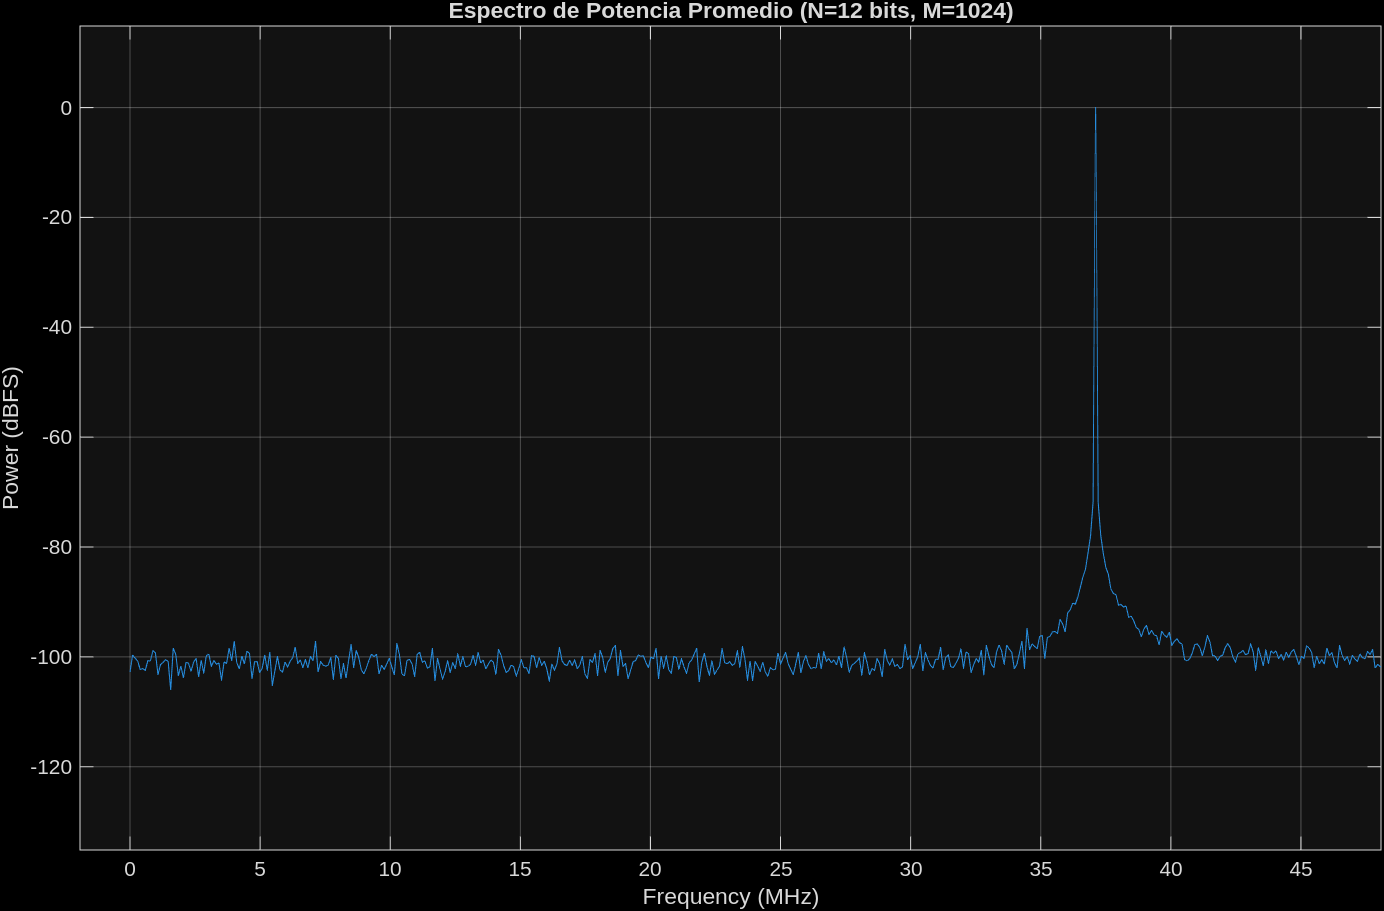
\includegraphics[width=1\textwidth]{img/task4_1.png}
    \label{fig:task4_1}
\end{figure}

On the figure we can see a signal peak at 37.1094 MHz, whith a value of 0 DBFS.

This agrees quantitatively with the theory, which predicts a peak at the input frequency.

$f_0 = 37.1094 MHz$ and a level of 0 dBFS due to the normalization used for a full-scale signal.

We can also see that the noise floor is around the 100 DBFS, which agrees with the theoretical value.
\vspace{1cm}

\textbf{Question: Repeat the previous steps for an FFT size M = 256.
}
\subsection{Theoretical values}
As the frequency $f_0$ is the same, we would also have a signal peak on that point.
Since is full-scale too, thew value of the peak would also be 0 DBFS.

The SQNR will be the same, because we have the same number of bits and the same $\sigma_x$.

However, the gain will change, as we have a different value for M.
$Gain = 10log_{10}(M/2) = 10log_{10}(256/2) = 21.07$

For M = 256 we will have a nois floor of 95.06 DBFS

\subsection{Matlab execution}
Executing the task\_4\_2.m script, we can see a noise peak of 0 DBFS at $f_0$ and a level of noise floor
of approximately 95 DBFS
\begin{figure}[H]
    \centering
    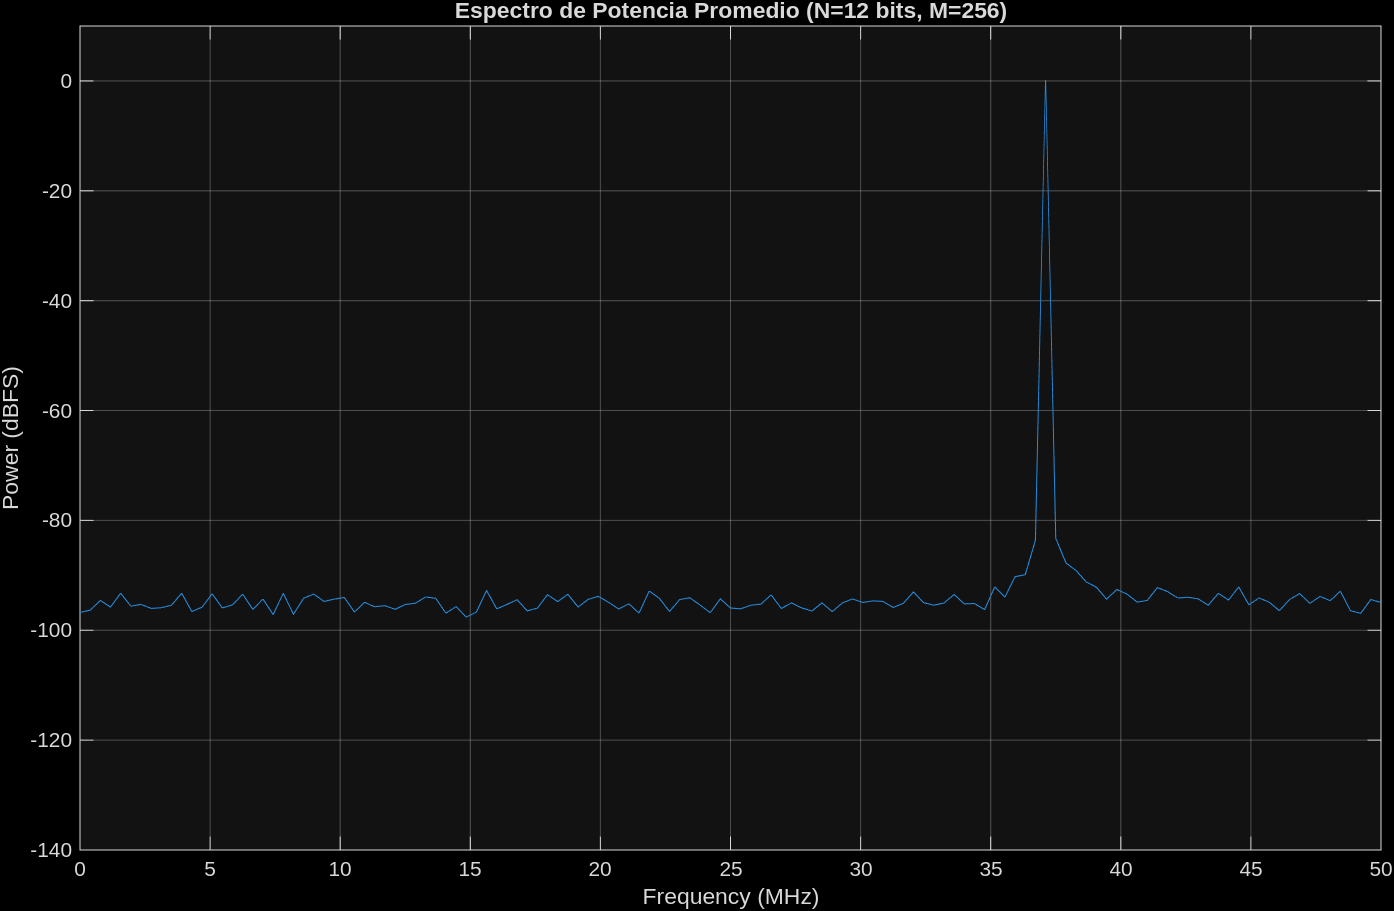
\includegraphics[width=1\textwidth]{img/task4_2.png}
    \label{fig:task4_2}
\end{figure}
\vspace{1cm}

\textbf{Question: Set again M = 1024, and repeat the analysis for decreasing resolutions of 10, 8 and 6 bits.}
\subsection{Theoretical values}

As the frequency $f_0$ is the same, we would also have a signal peak on that point.
Since is full-scale too, thew value of the peak would also be 0 DBFS.

The Gain will be the same as on task4\_1 because we have thje same M.

The SQNR will change, because we have different values for N:
\begin{itemize}
    \item N = 10: $SQNR = 6.02N +4.77 -20log_{10}(FS/\sigma_x) = 6.02 * 10 +4.77 -20log_{10}(\sqrt{2}) = 61.95 DBFS$
    \item N = 8: $SQNR = 6.02N +4.77 -20log_{10}(FS/\sigma_x) = 6.02 * 8 +4.77 -20log_{10}(\sqrt{2}) = 49.91 DBFS$
    \item N = 6: $SQNR = 6.02N +4.77 -20log_{10}(FS/\sigma_x) = 6.02 * 6 +4.77 -20log_{10}(\sqrt{2}) = 37.87 DBFS$
\end{itemize}

So the noise floor for each value of N will be:
\begin{itemize}
    \item N = 10: $-(61.95 + 27.09) = -89.04 DBFS $
    \item N = 8: $-(49.91 + 27.09) = -77 DBFS$
    \item N = 6: $-(37.87 + 27.09) = -64.96 DBFS$
\end{itemize}

\subsection{Matlab execution}

Executing the the task\_4\_3.m script, we can see three figures with a peak of 0 DBFS on $f_0$.
We also see a noise floor value of :
\begin{itemize}
    \item N = 10: $-89.05 DBFS $
    \item N = 8: $-77.01 DBFS$
    \item N = 6: $-64.97 DBFS$
\end{itemize}

\begin{figure}[H]
    \begin{subfigure}[t]{.5\textwidth}
        \centering
        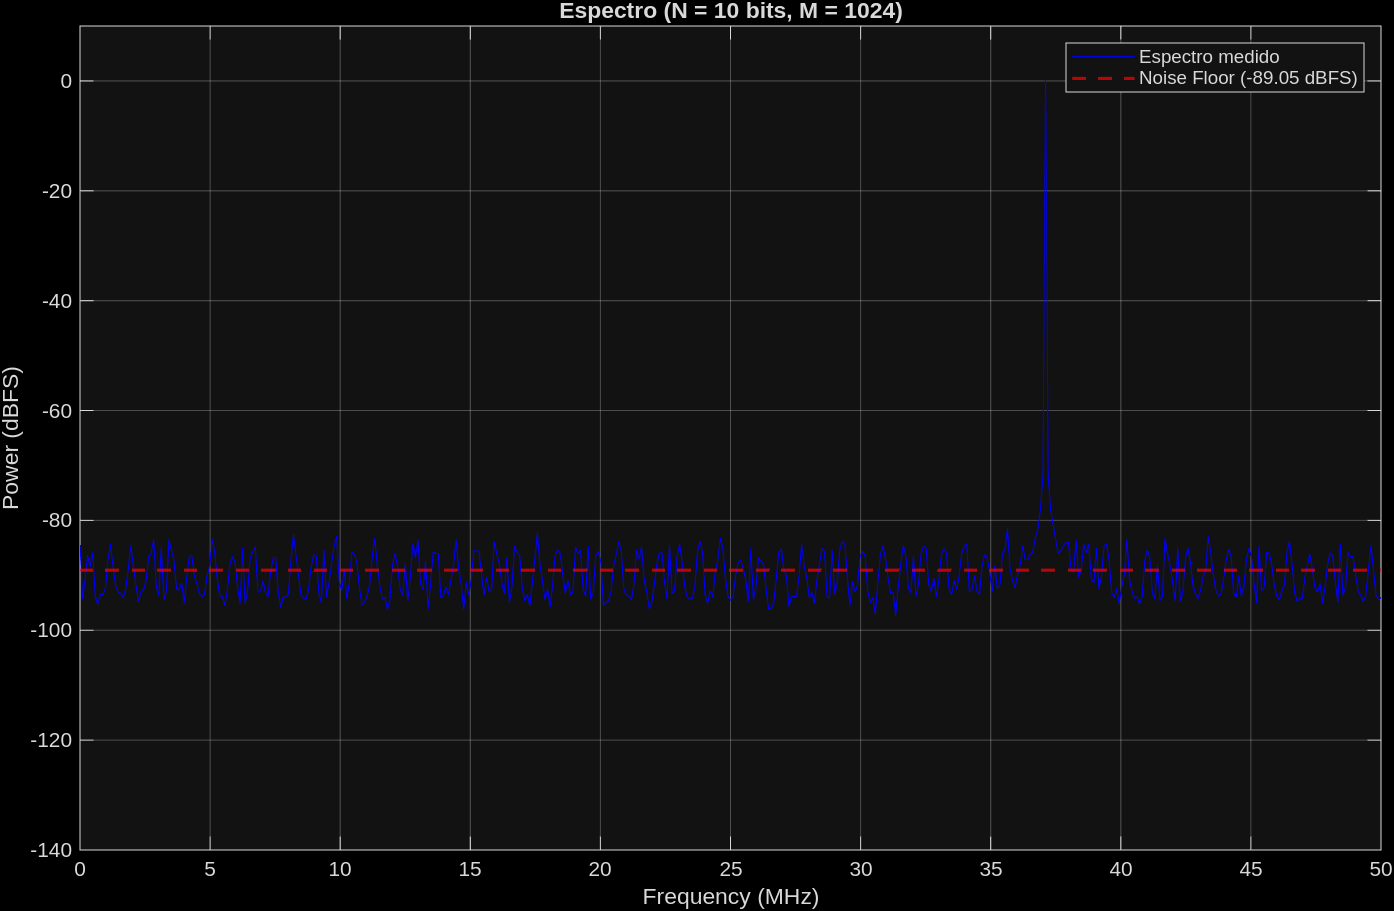
\includegraphics[width=\linewidth]{img/task4_3_n10.png}
        \caption{N=10 bits}
    \end{subfigure}
    \begin{subfigure}[t]{.5\textwidth}
        \centering
        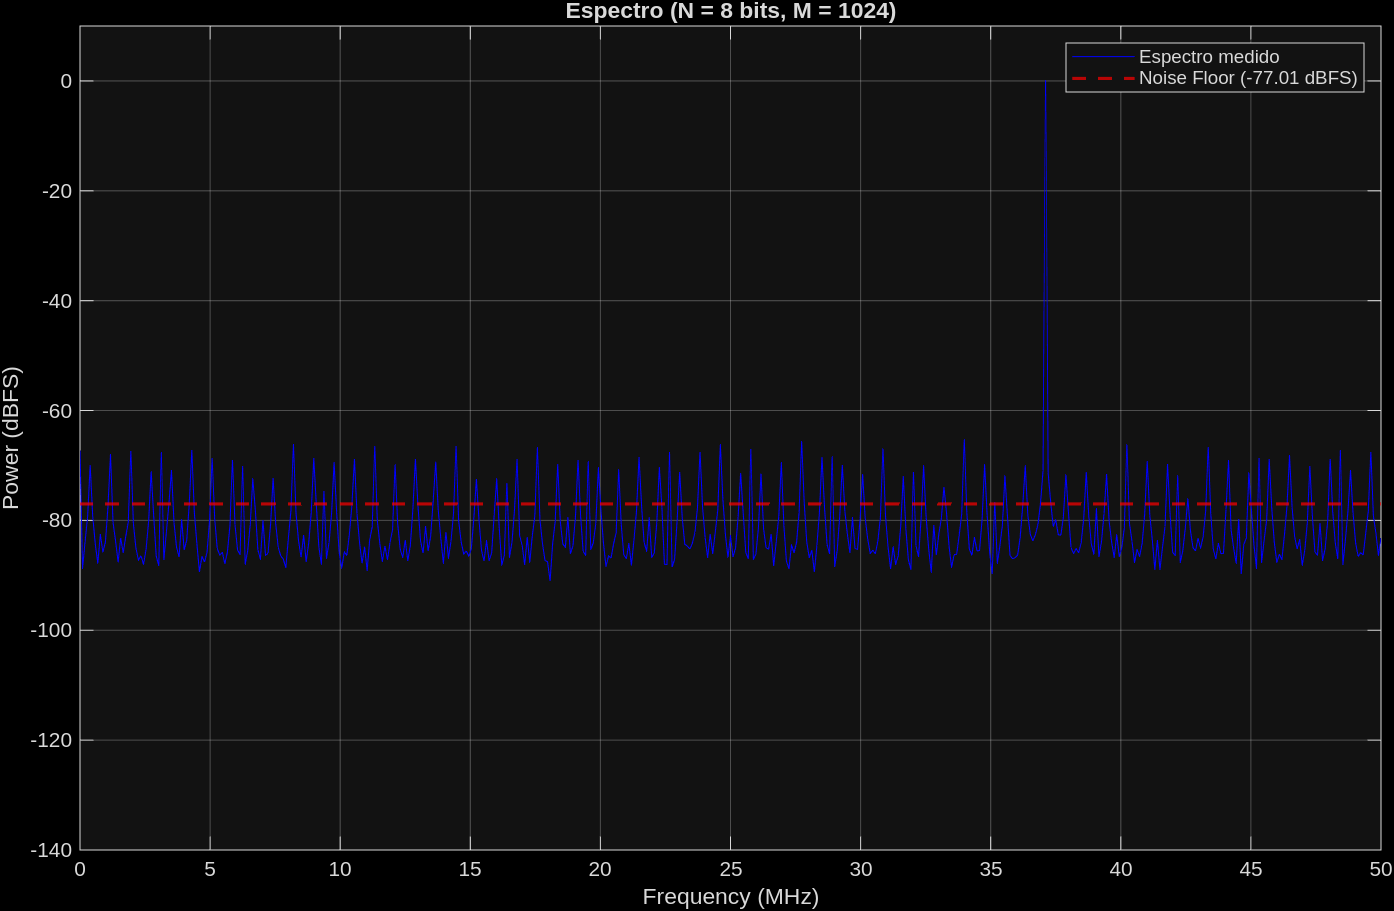
\includegraphics[width=\linewidth]{img/task4_3_n8.png}
        \caption{N=8 bits}
    \end{subfigure}
    \begin{subfigure}[t]{.5\textwidth}
        \centering
        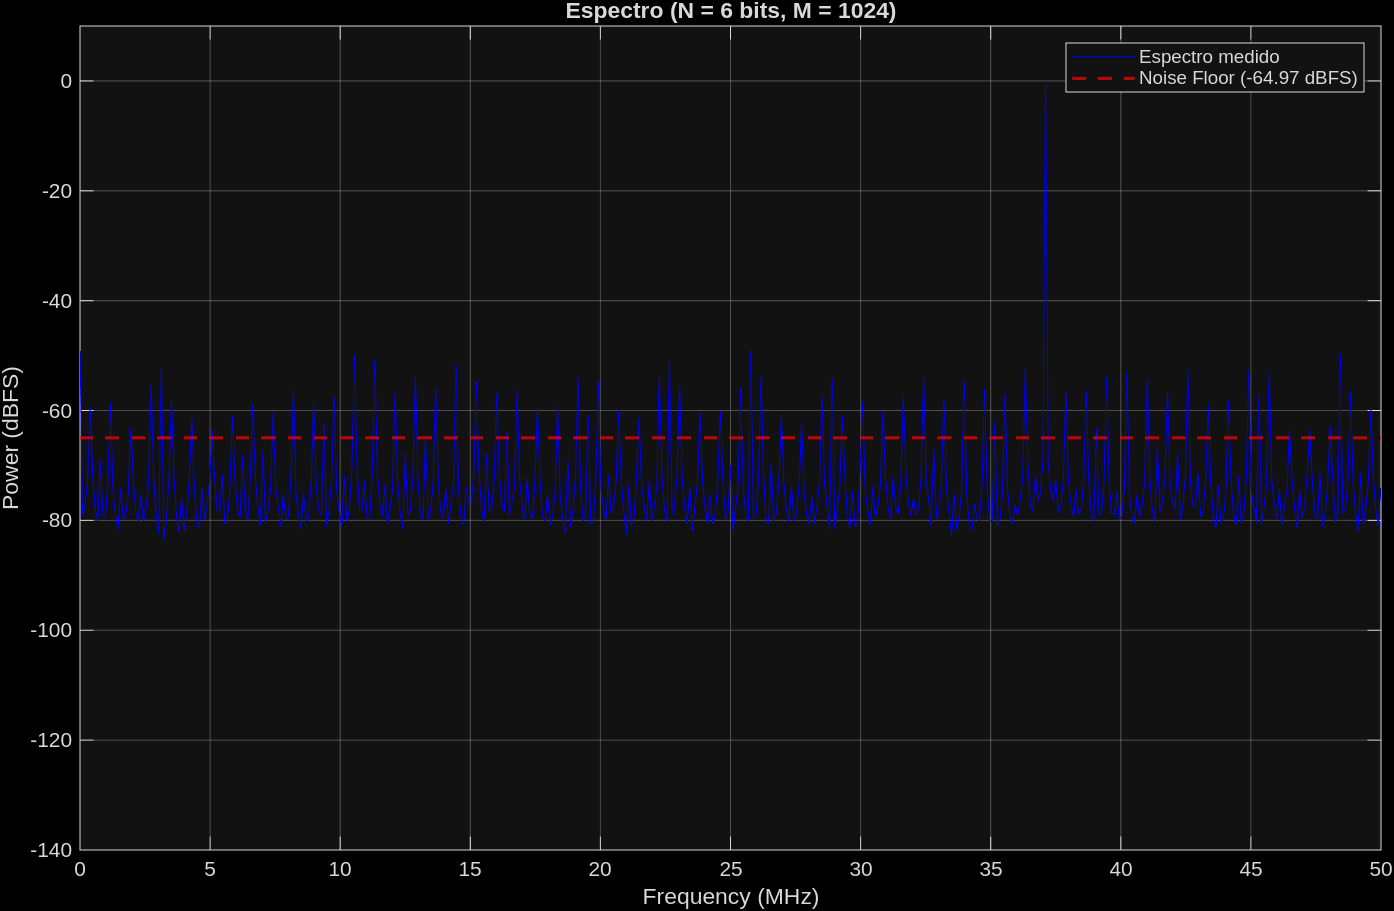
\includegraphics[width=\linewidth]{img/task4_3_n6.png}
        \caption{N=6 bits}
    \end{subfigure}
\end{figure}
\vspace{1cm}

\textbf{Question: Consider again M = 1024 and N = 12 bits. Repeat the analysis reducing the amplitude of
    the sinusoid to 1/3 of the full scale value, and compare your observations with the theoretical
    prediction.
}
\subsection{Theoretical values}
For a siusoid of amplitude $A =\alpha * FS , \alpha < 1$, we have $SQNR = 6.02N + 1,76 + 20log{10}(A)$.

For $A=1/3$ we have a SQNR of 64.81 DBFS. The gain will be the same, so we will have a noise floor of 91.9 DBFS


\vspace{1cm}

\textbf{Question: Let M = 1024, N = 12 bits and a full-scale sinusoid. Slightly change the frequency of the
    sinusoid to 37.12 MHz and repeat the analysis. How do your observations change? Does it make
    any difference if you use a larger number of samples, say 100 * M ? What happens if you increase
    the resolution to 16 bits?
    How do you explain all these?
}

The $f_0$ we had, was a $k$ of the FFT, so all the energy was on a single $k$: $ k =\frac{f_0*M}{fs} = \frac{37.1094*10^6*1024}{100*10^6}= 380$
When using the new frequency, the energy is between $k = 380$ and $k = 381$, so we see this power leak.

\begin{figure}[H]
    \centering
    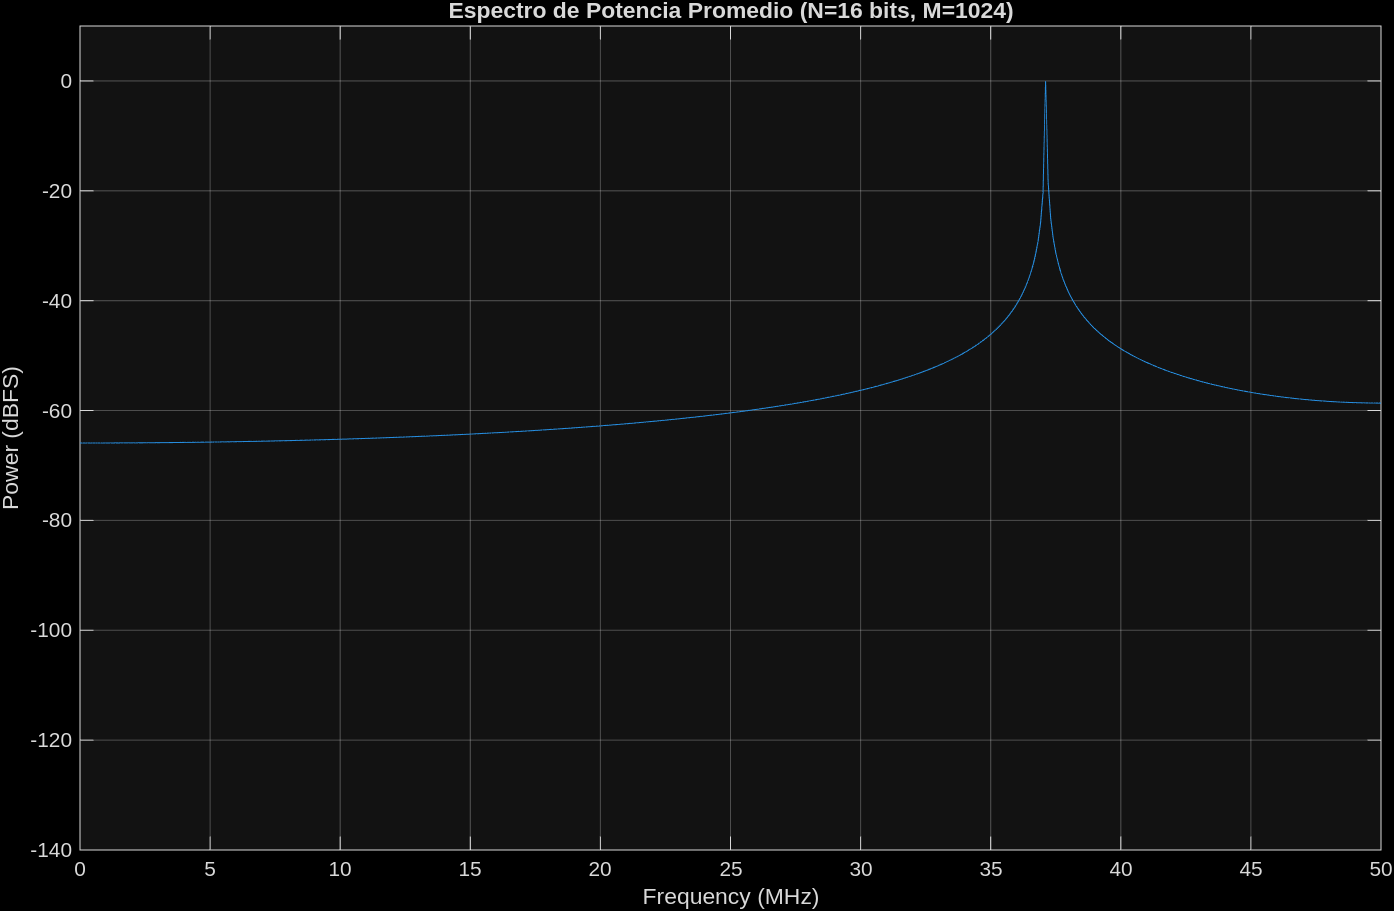
\includegraphics[width=1\textwidth]{img/task4_5.png}
    \label{fig:task4_5}
\end{figure}

Increasing the number of samples or the resolution will not have effect, because we need to have the signal on a $k$.
To do this, we can change either the $f_0$, the $fs$ or M.